\documentclass[12pt,a4paper]{article}
\renewcommand{\thesection}{\Roman{section}}
\renewcommand{\thesubsection}{\thesection.\Roman{subsection}}
\usepackage{xeCJK}
\usepackage{caption}
\usepackage{amssymb}
\usepackage{amsmath}
\usepackage{geometry}
\usepackage{subfigure}
\usepackage{fancyhdr}
\usepackage[export]{adjustbox}
\usepackage{graphicx}
\graphicspath{{images/}}
\geometry{left=2.5cm,right=1.5cm,top=2cm,bottom=2cm}

\title{Deep Learning and Practice \\Lab4 \\ Report}
\date{April 25, 2019}
\author{呂紹篁, 0751904}
\setCJKmainfont{AR PL UKai CN}
\begin{document}
\captionsetup[figure]{labelfont={bf},labelformat={default},labelsep=period,name={Fig.}}
\thispagestyle{plain}
\cfoot{}
\maketitle

\section{Intoduction} \label{sec:intro}
In this lab, we are aimed to implement 8-bit addition using \textbf{recurrent neural network (RNN)} from scratch. The optimized method is \textbf{backpropagation through time (BPTT)} and its mathematical derivation is pretty clear in the lecture. The restriction is that we can use only pure Python or with the help of Numpy.

\section{Experiment Setups} \label{sec:exp_setup}
\subsection{Recurrent Neural Network}
Convolution neural network (CNN) is pretty strong to do work such as signal processing (Lab 1, 2), image classification (Lab 3) and dense segmentation (fully convolution network, FCN). While the common part mentioned above is that the data is not a \textbf{time sequence}, i.e, the data and its neighbor are independent in some sense. This is, however, not suitable for data that related to time, such as \textbf{natural language}. Take a simple example, if I say "I am hungry", then the sentence I say next may more likely be "what can I eat?" rather than "the lab this time is so difficult". For data with this features, it is more suitable for training using RNN, since the network also consider the correlation inside the data, the binary addition task this time is a nice example, where the digits behind may bring carry information.
The architecture of the RNN in this lab is illustrated in Fig. \ref{fig:rnn}. \\
\begin{equation}
\begin{cases}

&\textbf{W} \in \mathbb{R}^{m\times m} \text{ is a transition matrix between hidden units } h^{(t)}  \\
&\textbf{U} \in \mathbb{R}^{m\times k} \text{ is a transition matrix mapping from input } x^{(t)} \text{ to hidden units} \\
&\textbf{V} \in \mathbb{R}^{n\times m} \text{ is a transition matrix from hidden units to output units } o^{(t)}\\
&x^{(t)} \in \mathbb{R}^{k\times 1} \text{ is called input unit}\\
&h^{(t)} \in \mathbb{R}^{m\times n} \text{ is called hidden unit}\\
&o^{(t)} \in \mathbb{R}^{m\times n} \text{ is called output unit}\\
\end{cases}
\end{equation}
% k2 m16 n1
In this lab, k equals to 2 (two input channel), m equals to 16 and n equals to 1 (either 0 or 1). The relation between each unit are summarized as following, which are the \textbf{forward propagation} of our network: % forward 
\begin{equation}
\begin{cases}
& a^{(t)} = Wh^{(t-1)}+Ux^{(t)} \\
& h^{(t)} = \sigma (a^{t)}) \\
& o^{(t)} = Vh^{(t)} \\
& y_{pred}^{(t)} = \sigma ({o^{(t)}}) \\
\end{cases}
\end{equation}
$h^{(0)}$ stands the initial vector and can be given arbitrary, in this work, we simply used zero vector.
To simplify the code, we neglected bias terms in the lecture, and since this is a logistic regression problem, we used \textbf{sigmoid} as activation function to make output unit in range (0, 1). For evaluation, we used \textbf{cross entropy} as Lab 1 mentioned. 

\subsection{Training Data Generation}
To generate training data, we prebuilt a binary list from range 0 to 255, i.e., [0,0,0,0,0,0,0,0] to [1,1,1,1,1,1,1,1]. For each iteration, we randomly choose two intergers from range [0, 128), find their corresponding binary representation and feed as input data from LSB to MSB.

\subsection{BPTT for Updating Weights}
The equations for updating weights are summarized as following:
\begin{equation}
\begin{cases}
& \nabla_{\textbf{W}}L = \sum_{t}{H^{(t)}(\nabla_{h^{(t)}} L)h^{(t-1)T}}\\
& \nabla_{\textbf{U}}L = \sum_{t}{H^{(t)}(\nabla_{h^{(t)}} L)x^{(t)T}}\\ 
& \nabla_{\textbf{V}}L = \sum_{t}(\nabla_{o^{(t)}}L) h^{(t)T} \\
& \nabla_{{h^{(t)}}}L = \textbf{W}^T H^{(t+1)} V^T (\nabla_{o^{(t+1)}}L)+ V^T (\nabla_{o^{(t)}}L)\\
& \nabla_{o^{(t)}}L = y_{pred} - y \\
& H^{(t)} = \frac{\partial{h^{(t)}}}{\partial{a^{(t)}}} \\
\end{cases}
\label{equ:bptt}
\end{equation}
Notice that the fourth equation in (\ref{equ:bptt}) consider the next time stamp, for last t (in this lab, t=8), we can simply neglect the term.
\subsection{Code Overview}
The code can break into two parts: training and testing. For testing, we used the model we trained to test the addition. For training, it can break into forward and backward parts, to implement the BPTT as equation above, in forward phase we saved the result of hidden units, ground truth and predicted results. We predict the result from LSB to MSB as human do addition.

\begin{figure}[hbt]
\centering
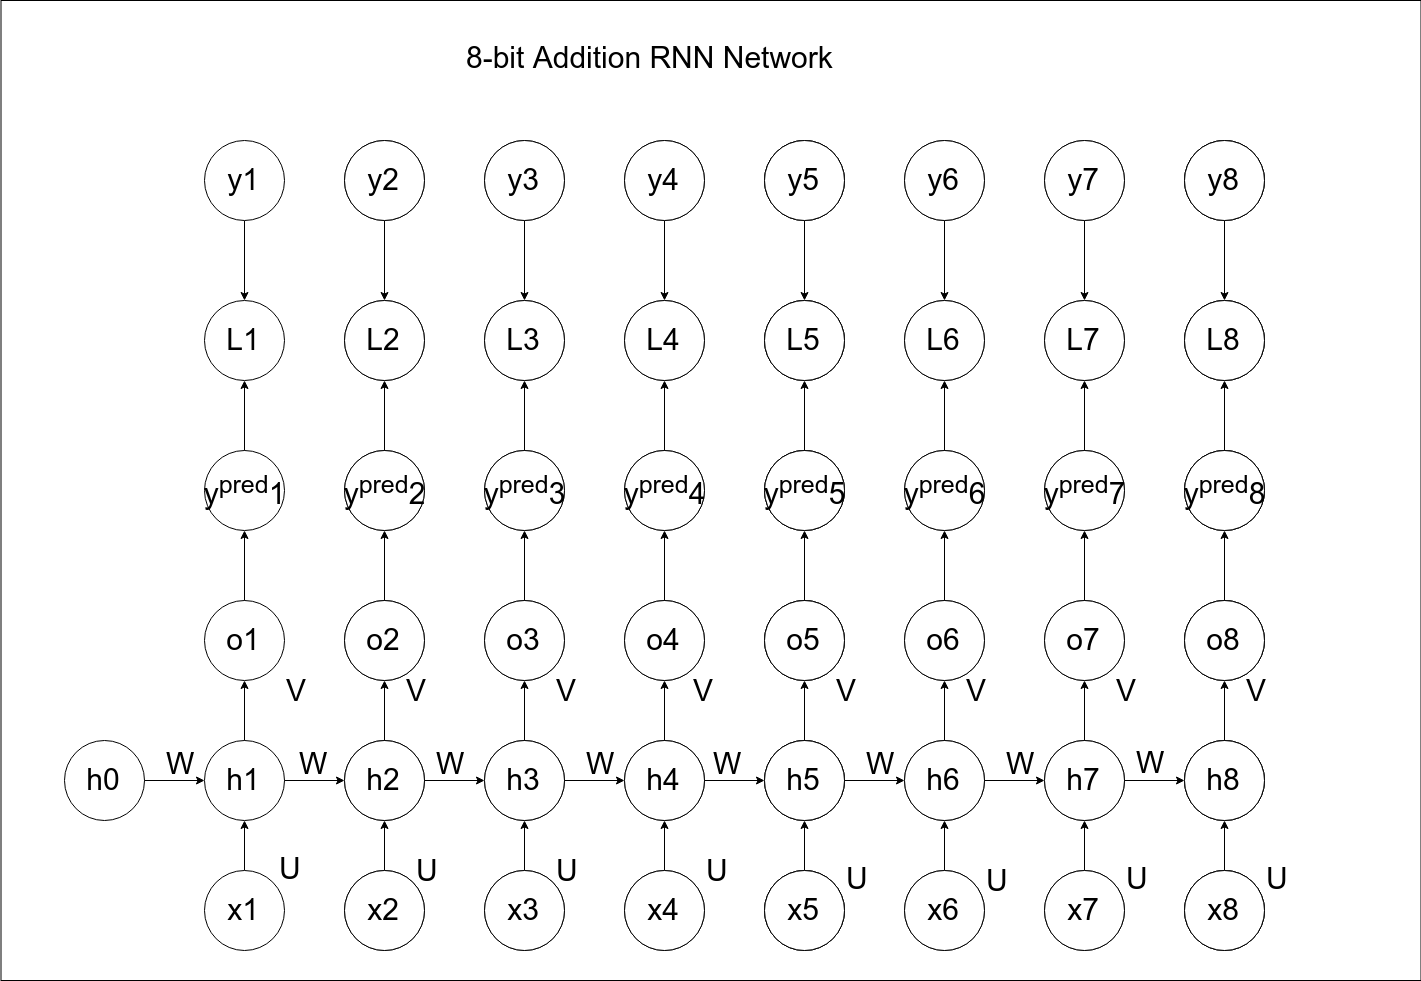
\includegraphics[scale=0.3]{rnn.png}
\caption{RNN Archietecture}
\label{fig:rnn}
\end{figure} 


\section{Experimental Results} \label{sec:res}
The training accuracy curve is illustrated in Fig. \ref{fig:acc}. It is shown that the accuracy approached 100 percent right after less than 3000 iterations. As TA mentioned, the loss can decrease rapidly if we update the weights correctly. (Fig. \ref{fig:loss})

\begin{figure}[hbt]
\centering
\subfigure[Training Accuracy Curve]{
  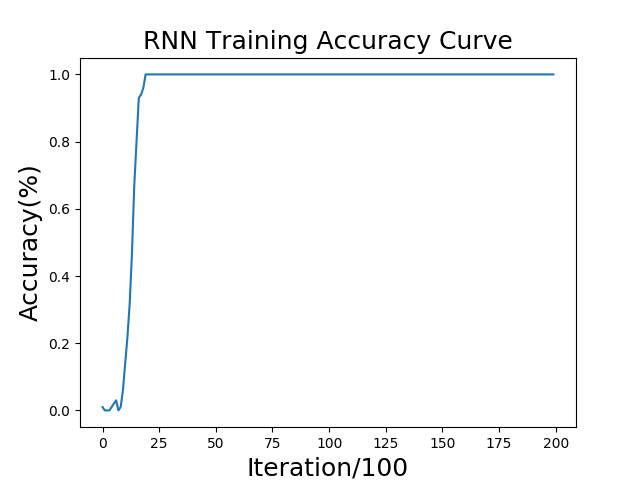
\includegraphics[scale=0.5]{acc.png}
  \label{fig:acc}
}
\subfigure[Loss Curve]{
  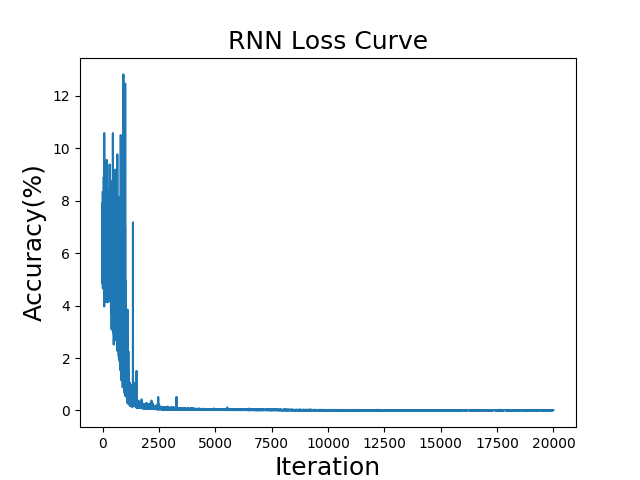
\includegraphics[scale=0.5]{loss.png}
  \label{fig:loss}
}
\end{figure} 

\section{Discussion} \label{sec:dis}
\begin{itemize}
\item {Signed 8-bit Addition?} \\
After completing unsigned 8-bit addition, we further consider signed one. The code (which is provided in $\text{lab4\_neg.py}$) is almost the same besides conversion between two representation and data generation part: since including negative part, MSB this time doesnot effect the magnitude and hence the range becomes [-128, 127]. Two random intergers should choose in range [-64, 64) to prevent overfloat. The weird behavior is that though the accuracy in training phase is remained low (about 50\%), in test phase it still got 100\% accuracy which shown that the network learned both addition and subtraction. 

\end{itemize}


%\bibliographystyle{IEEEtran}
%\bibliography{report.bib}

\end{document}
